% !TEX TS-program = pdflatex
% !TEX encoding = UTF-8 Unicode

% This file is a template using the "beamer" package to create slides for a talk or presentation
% - Giving a talk on some subject.
% - The talk is between 15min and 45min long.
% - Style is ornate.

% MODIFIED by Jonathan Kew, 2008-07-06
% The header comments and encoding in this file were modified for inclusion with TeXworks.
% The content is otherwise unchanged from the original distributed with the beamer package.

\documentclass{beamer}


% Copyright 2004 by Till Tantau <tantau@users.sourceforge.net>.
%
% In principle, this file can be redistributed and/or modified under
% the terms of the GNU Public License, version 2.
%
% However, this file is supposed to be a template to be modified
% for your own needs. For this reason, if you use this file as a
% template and not specifically distribute it as part of a another
% package/program, I grant the extra permission to freely copy and
% modify this file as you see fit and even to delete this copyright
% notice. 


\mode<presentation>
{
  \usetheme{Warsaw}
  % or ...

  \setbeamercovered{transparent}
  % or whatever (possibly just delete it)
}


\usepackage[english]{babel}
% or whatever

\usepackage[utf8]{inputenc}
% or whatever

\usepackage{times}
\usepackage[T1]{fontenc}
\RequirePackage[numbers,sort&compress,square,comma]{natbib}
\bibliographystyle{IEEEtranN}
% Or whatever. Note that the encoding and the font should match. If T1
% does not look nice, try deleting the line with the fontenc.


\title[Quantum Dots with Primitives] % (optional, use only with long paper titles)
{Modeling Quantum Dots using Geometric Primitives}

\subtitle
{} % (optional)

\author[] % (optional, use only with lots of authors)
{J. M. Calderon}
% - Use the \inst{?} command only if the authors have different
%   affiliation.

\institute[University of York] % (optional, but mostly needed)
{%
  Department of Computer Science\\
  University of York
 }
% - Use the \inst command only if there are several affiliations.
% - Keep it simple, no one is interested in your street address.

\date[] % (optional)
{19-9-2011 / MSc NC Presentation}

\subject{Talks}
% This is only inserted into the PDF information catalog. Can be left
% out. 



% If you have a file called "university-logo-filename.xxx", where xxx
% is a graphic format that can be processed by latex or pdflatex,
% resp., then you can add a logo as follows:

% \pgfdeclareimage[height=0.5cm]{university-logo}{university-logo-filename}
% \logo{\pgfuseimage{university-logo}}



% Delete this, if you do not want the table of contents to pop up at
% the beginning of each subsection:
\AtBeginSubsection[]
{
  \begin{frame}<beamer>{Outline}
    \tableofcontents[currentsection,currentsubsection]
  \end{frame}
}


% If you wish to uncover everything in a step-wise fashion, uncomment
% the following command: 

%\beamerdefaultoverlayspecification{<+->}


\begin{document}

\begin{frame}
  \titlepage
\end{frame}

\begin{frame}{Outline}
  \tableofcontents
  % You might wish to add the option [pausesections]
\end{frame}


% Since this a solution template for a generic talk, very little can
% be said about how it should be structured. However, the talk length
% of between 15min and 45min and the theme suggest that you stick to
% the following rules:  

% - Exactly two or three sections (other than the summary).
% - At *most* three subsections per section.
% - Talk about 30s to 2min per frame. So there should be between about
%   15 and 30 frames, all told.

\section{Introduction}

\subsection[What are Quantum Dots?]{Explaining Quantum Dots}

\begin{frame}
The Sch\"{o}dinger Equation

\begin{equation}
E\psi = -\frac{\hbar ^2}{2m}\nabla ^2 \psi + V\psi \nonumber
\label{eq:timeIndependent2}
\end{equation}

Where

\begin{equation}
\nabla ^2 =  \left(\frac{\partial ^2}{\partial x} + \frac{\partial ^2}{\partial y} + \frac{\partial ^2}{\partial z}\right) \nonumber
\label{eq:laplace}
\end{equation}
and
$$\psi \rightarrow \text{the wave equation for the particle}$$
\end{frame}

\begin{frame}[fragile]{Understanding Potential Wells}{Potential Wells}
   Free particles like to reside where the potential energy is low

\begin{figure}[h]
  \centering
  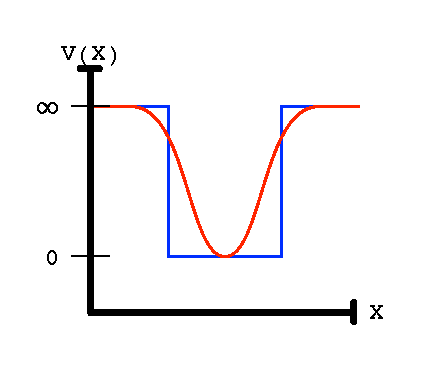
\includegraphics[scale=0.7]{figures/realWell.eps}
\end{figure}
  Normally a function describing this function can be complex (the red line), so physicists
  approximate it using a trivial function to make things easier (blue line) \cite{dots}.
\end{frame}

\begin{frame}[fragile]{Quantum Confinement}{}
  Infinitely deep well $\rightarrow$ quantum confinement 

\begin{figure}[h]
 \centering
 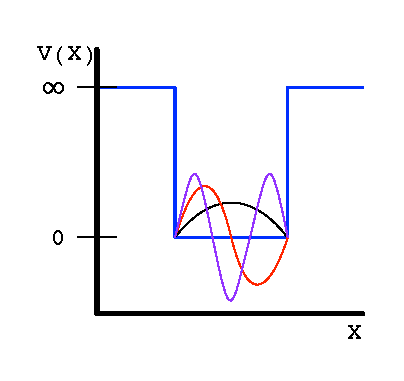
\includegraphics[scale=.7]{figures/confined.eps}
\end{figure}
\end{frame}


\begin{frame}{Quantum Dots as Artificial Atoms}{}
  % - A title should summarize the slide in an understandable fashion
  %   for anyone how does not follow everything on the slide itself.

  Quantum Confinement in 3D -> Artificial atom
  \begin{itemize}
  \item
   Question: What atomic properties are we looking to exploit?
   \pause
  \item
    Answer: Fluorescence.
  \end{itemize}
\end{frame}

\begin{frame}[fragile]{Fluorescence}{Fluorescence 1}
  How fluorescence works

\begin{figure}[h]
 \centering
 \includegraphics[scale=0.7]{figures/atomEnergies.eps}
\end{figure}
A photon `hits' an electron into its excited state.
\end{frame}
\begin{frame}[fragile]{Fluorescence}{Fluorescence 2}
  How fluorescence works

\begin{figure}[h]
 \centering
 \includegraphics[scale=0.7]{figures/flourece.eps}
\end{figure}
When the electron comes back `down' form the excited state
light is emitted \cite{qp}. 
\end{frame}


\section{Method}
\subsection{Approximating the kinetic energy}
\begin{frame}
Remembering the Schr\"{o}dinger equation

\begin{equation}
E\psi = -\frac{\hbar ^2}{2m}\nabla ^2 \psi + V\psi \nonumber
\label{eq:timeIndependent2}
\end{equation}

Let us first model the kinetic energy part

$$K = -\frac{\hbar ^2}{2m}\nabla ^2$$

where

$$
\nabla ^2 =  \left(\frac{\partial ^2}{\partial x} + \frac{\partial ^2}{\partial y} + \frac{\partial ^2}{\partial z}\right) \nonumber
$$
\end{frame}

\begin{frame}
$$f'(x) \approx \frac{f(x + h) - f(x)}{h}$$
and 
$$f''(x) \approx \frac{f(x + h) - 2f(x) + f(x - h)}{h^2}$$
\end{frame}

\begin{frame}
This gives us the following matrix for $f''(x)$
\begin{equation}
\begin{bmatrix}
                -2     &   1    &     0    &     0   & \cdots & 0 \\
                1      &  -2    &     1    &     0   & \cdots & 0 \\
                0      &   1    &    -2    &     1   & \cdots & 0 \\
                \vdots & \vdots &   \vdots & \vdots  & \ddots & \vdots \\
                0      & \cdots &    \cdots     &     0   &    1   & -2
              \end{bmatrix}  \nonumber
\end{equation}
\end{frame}

\begin{frame}
This works fine for a one dimensional function like this one
\begin{figure}[h]
  \centering
  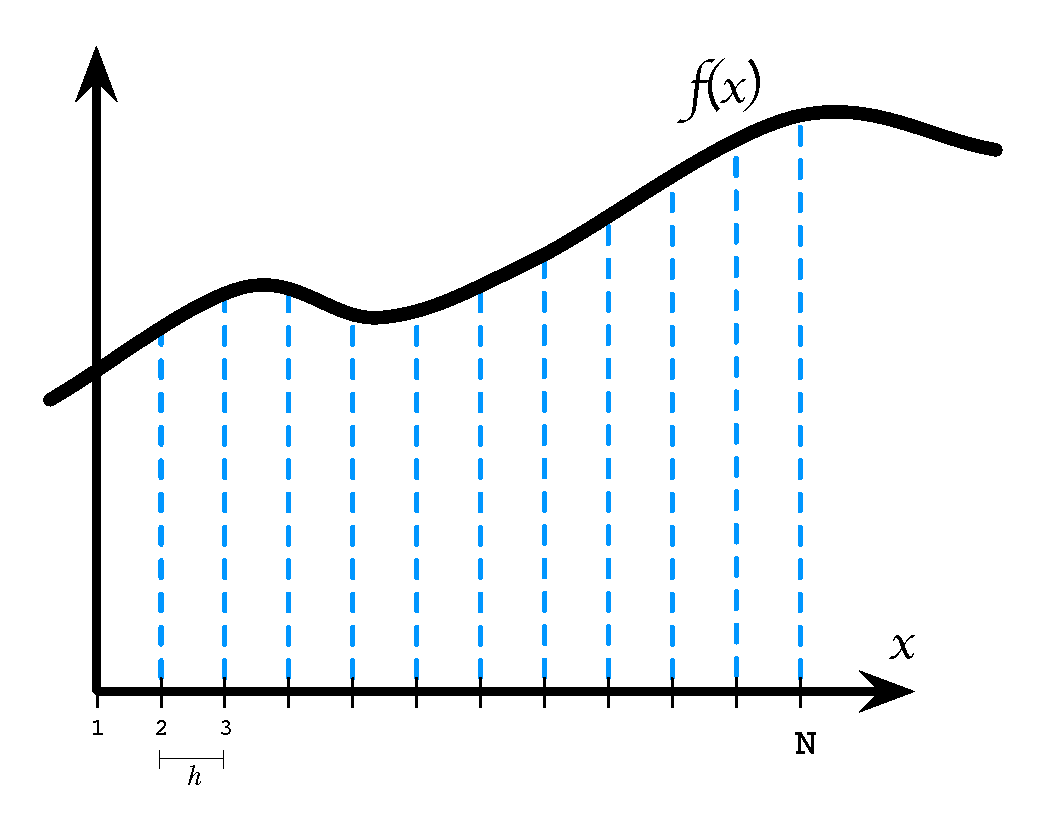
\includegraphics[scale=0.3]{figures/sampledFunc3.eps}
\end{figure}

But what about higher dimensionality?
\end{frame}

\begin{frame}
This is what we want!
\begin{figure}
\centering
  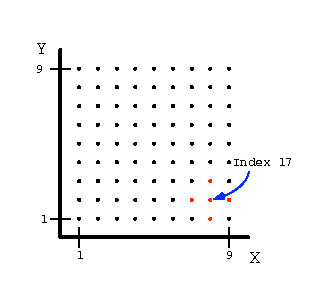
\includegraphics[scale=1.2]{figures/finite2D.eps}
\label{fig:finite2D}
\end{figure}
\end{frame}

\begin{frame}
Luckily, we can use the tensor product to achieve this. 

For 2 dimensions
\begin{equation}
K = X \otimes I + I \otimes Y \nonumber
\end{equation}
For 3 dimensions
\begin{equation}
K = X \otimes I \otimes I + I \otimes Y \otimes I + I \otimes I \otimes Z \nonumber
\end{equation}
This process gives us the appropriate approximation of the kinetic energy matrix. 
\end{frame}

\subsection{Potential Energy Matrix}

\begin{frame}
Now we can create our potential energy matrix. 

\begin{itemize}
  \item Have a set of defined primitives
  \item Iterate through the set of sample points
  \item For each point determine if it is inside any of the primitves
  \item Place results along the diagonal of a matrix.
\end{itemize}
\end{frame}

\begin{frame}
  Set of primitives
    \begin{itemize}
      \item Sphere
      \item Rectangular Prism
      \item Cylinder
    \end{itemize}
\end{frame}

\begin{frame}
Determining if a point is inside a prism
\begin{figure}[h!]
  \centering
  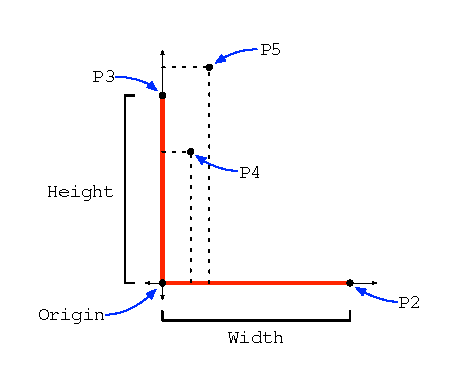
\includegraphics[scale=1.2]{figures/recPrism.eps}
\end{figure}
\end{frame}

\subsection{Combining The Two}
\begin{frame}
Now that we have both matrices we can add them together and solve for the eigenvalues.

$$E\psi = K \psi + V \psi$$

The eigenvalues of $E$ codify the spectral information of the quantum dot. 
\end{frame}

\section{Results}
\subsection{Results}
\begin{frame}
Having an implementation, we can now compare its results to an analytical solution (of a very simple case).

Two comparisons can be made

\begin{itemize}
 \item First ten eigenvalues should be $3,6,6,6,9,9,9,11,11,11$
 \item For a cube of $.8$ the length of the sample cube, the lowest eigenvalue should be $46.2638$
\end{itemize}
\end{frame}


\begin{frame}[fragile]
Percent error of the first ten eigenvalues (increasing the sample rate)
\begin{figure}
\centering
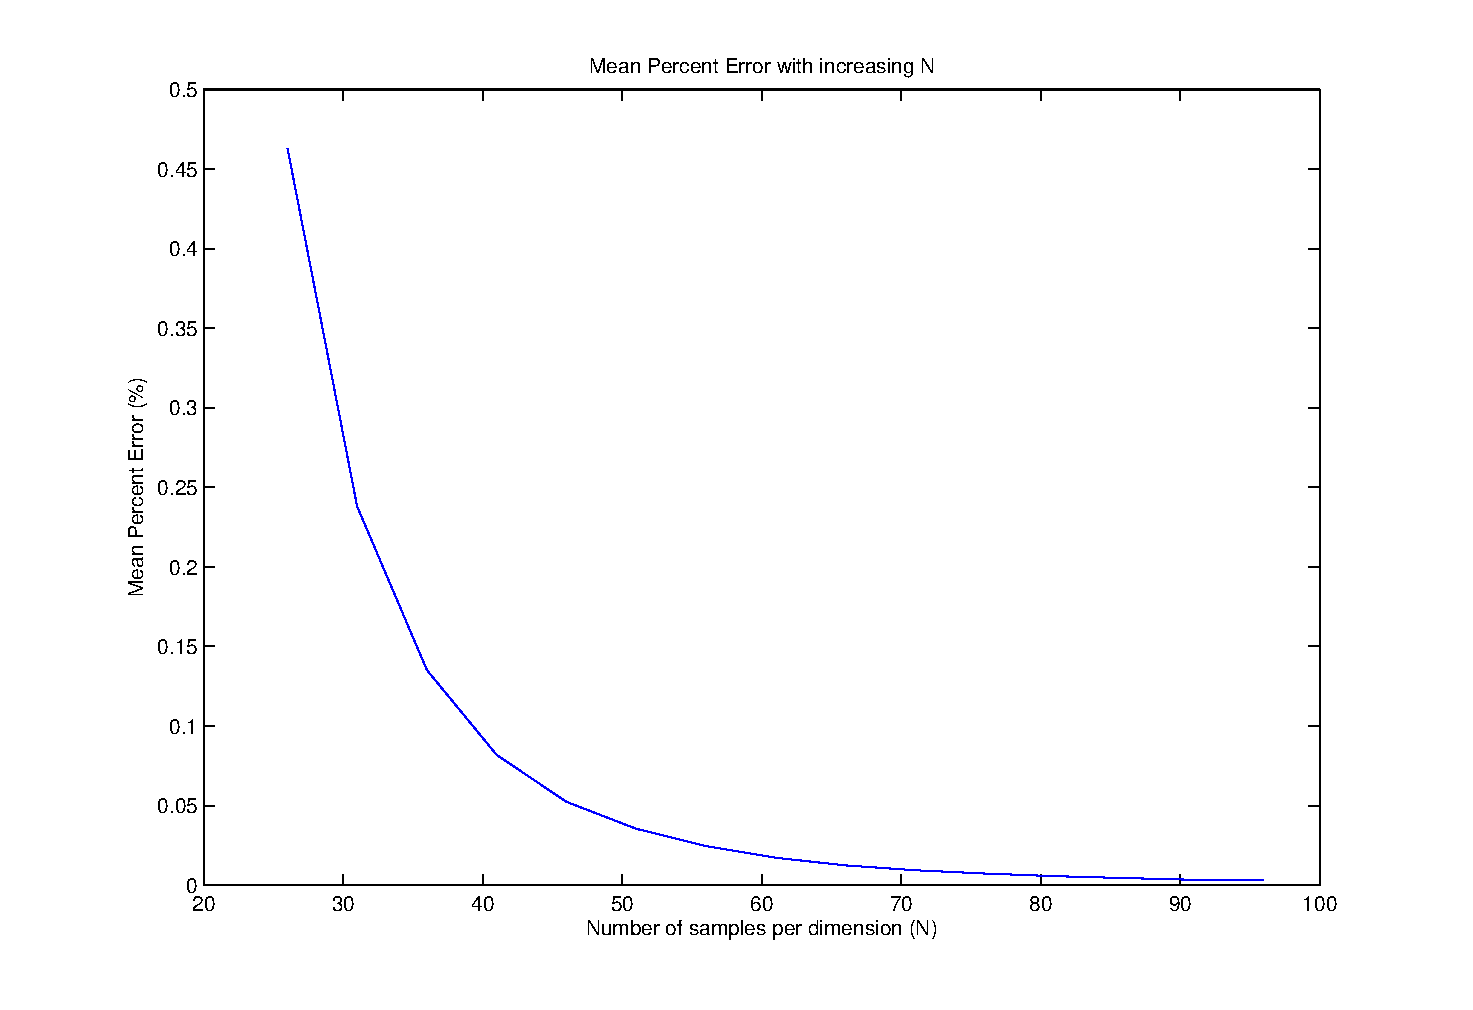
\includegraphics[scale=0.4]{figures/meanPercentError.eps}
\end{figure}
\end{frame}

\begin{frame}
Value of first eigenvalue with cube of $.8$ the length of the sample cube.
\begin{figure}[!h]
\centering
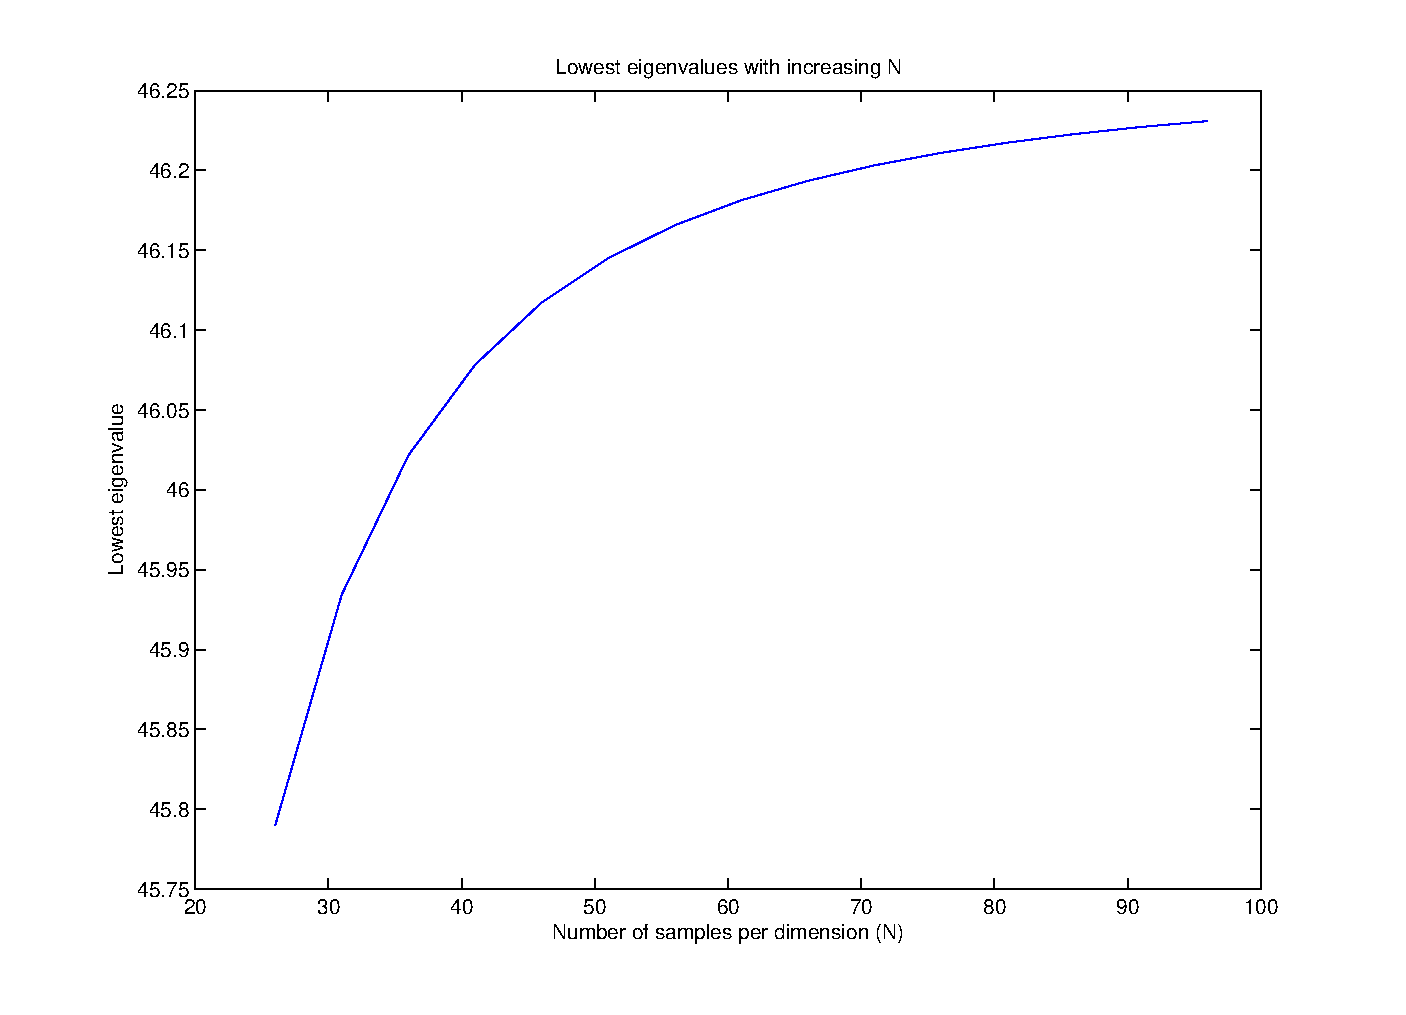
\includegraphics[scale=0.4]{figures/M2converge.eps}
\end{figure}
\end{frame}

\section*{Conclusion}

\begin{frame}{Conclusion}

  % Keep the summary *very short*.
  \begin{itemize}
  \item
   By using primitives we can abstract away from the sample-point level.
  \item
   Using the approximation methods based on the Taylor series provides a simple 
   yet effective approximation of the energy levels.
  \item
   Finding computers that had sufficient memory resources proved to be a problem.
  \end{itemize}
  
  % The following outlook is optional.
  \vskip0pt plus.5fill
  \begin{itemize}
  \item
    Outlook
    \begin{itemize}
    \item
     Run more tests, including the variation of the potential field (changing the surrounding electric field)
    \item
     Use this to create an evolutionary algorithm to find optimal shapes for desired spectral properties.
    \end{itemize}
  \end{itemize}
\end{frame}

\section*{Questions}

\begin{frame}
\centering
Questions
\end{frame}
\bibliography{diss}

\end{document}


